\section{Face Detection}

\subsection{Preprocessing for Eigenface Computation}

In the directory \texttt{hw2\_materials\_f20/problem3} you can find a folder named \texttt{lfw1000}, which contains 1071 face images. Each of these images is a $64 \times 64$ gray scale image. Figure \ref{face_example} shows some examples.


\begin{figure}[h!]
    \centering
    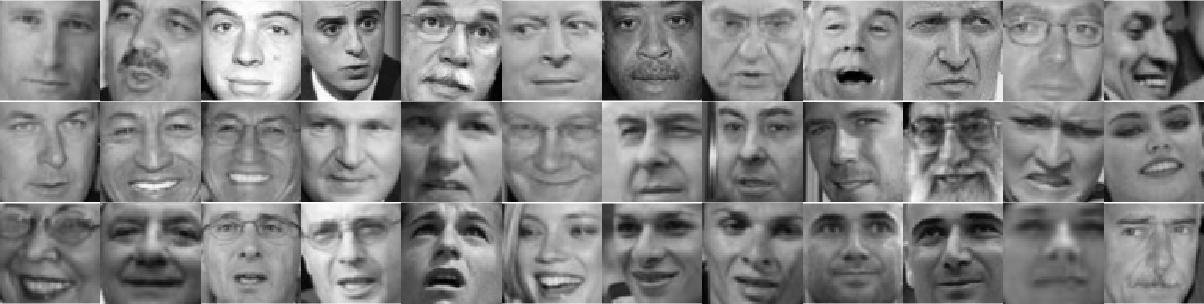
\includegraphics[scale=0.35]{figs/faces.jpg}
    \caption{Examples of face images.}
    \label{face_example}
\end{figure}


The Matlab (top) and Python (bottom) command to read an image is:
\begin{lstlisting}
image = double(imread(imagefile));
-------------------------------------------------------------------------------------------------
from PIL import Image
image = Image.open(imagefile)
\end{lstlisting}
Note we are using \texttt{double()}. If you do not use it, Matlab reads the data as \texttt{uint8} and some operations cannot be performed.


We consider that each face can be approximated by a linear combination of eigenfaces, that is, each face $F$ can be approximated as
\begin{equation}
  F \approx \omega_{F,1}E_1 + \omega_{F,2}E_2 +...+\omega_{F,k}E_k  
\end{equation}\\
where $E_i$ is the $i^{\text{th}}$ eigenface and $\omega_{F,i}$ is the weight of the $i^{\text{th}}$ eigenface when composing face $F$. 

To learn eigenvectors, the collection of faces must be unravelled into a matrix. To unravel an image of any size, you can do the following:
\begin{lstlisting}
[nrows, ncolumns] = size(image);
image = image(:);
-------------------------------------------------------------------------------------------------
import numpy as np
nrows, ncolumns = image.height, image.width
image = np.asarray(image.getdata())
\end{lstlisting}
The first line above is used only to retain the size of the original image. We will need it to fold an
unravelled image back into a rectangular image. The second line converts the \texttt{nrows} $\times$ \texttt{ncolumns} image into
a single \texttt{nrows}$\cdot$\texttt{ncolums} $\times$ $1$ vector. 
To read in an entire collection of images, you can do the following:
\begin{lstlisting}
filenames = textread('FILE WITH LIST OF IMAGE FILE NAMES','%s');
nimages = length(filenames);
for i = 1:nimages
    image{i} = double(imread(filenames{i}));
end
-------------------------------------------------------------------------------------------------
import os
for i, filename in enumerate(os.listdir(imagedirectory)):
    image = Image.open(os.path.join(imagedirectory, imagefile))
    X[:,i] = np.asarray(image.getdata())
\end{lstlisting}

To compose matrix from a collection of \texttt{k} images, the following Matlab script can be employed (you can also do it your own way, not necessary if using the Python script above):
\begin{lstlisting}
X = [];
for i = 1:k
    X = [X image{i}(:)];
end
\end{lstlisting}

Eigenfaces can be computed from \texttt{X}, which is an (\texttt{nrows} $\cdot$ \texttt{ncolumns}) $\times$ \texttt{nimages} matrix. You will extract eigenfaces using three different basis representations in the following sections. \ul{Nothing needs to be submitted for this section}.

\subsection{Computing Eigenfaces with PCA}

For this part of the assignment, you will extract eigenfaces using PCA, which employs singular value decomposition to project the faces onto orthogonal bases (in Matlab, you can use the command \texttt{svd}; in Python, \texttt{np.linalg.svd}).

Each resulting eigenface will be in the form of a (\texttt{nrows} $\cdot$ \texttt{ncolumns}) $\times$ $1$ vector. To convert it to an image, you must
fold it into a rectangle of the right size. Matlab will do it for you with:
\begin{lstlisting}
eigenfaceimage = reshape(eigenfacevector, nrows, ncolumns);
-------------------------------------------------------------------------------------------------
eigenfaceimage = eigenfacevector.reshape(nrows, ncolumns)
\end{lstlisting}
\texttt{nrows} and \texttt{ncolumns} are the values obtained when you read the image. \texttt{eigenfacevector} is the eigenvector obtained from the eigenanalysis (or SVD).

\begin{enumerate}
    \item \textbf{First Eigenface}. 
    
    Using these 1071 images, \ul{find the first eigenface and plot it in your report} (you can use the Matlab command \texttt{imagesc} or the Pyplot command \texttt{plt.imshow()}). \ul{Submit the first eigenface as a $4096 \times 1$ vector in a file named \texttt{eigenface.csv}}.
    
    \item \textbf{Reconstruction Error}. 
    
    Given a face $F$ and the first $k$ eigenfaces, we can compute its reconstruction error as
    \begin{equation}
     \mathcal{E}(F \; ; \; E_1,...,E_k) = \left\| F - \sum_{i=1}^k \omega_{F,i} E_i \right\|_2
    \end{equation}
    
    Then, if we have $N$ faces, the mean reconstruction error is given by
    \begin{equation}
        \frac{1}{N} \sum_{j=1}^N \mathcal{E}(F_j \; ; \; E_1,...,E_k)
    \end{equation}
     
    Using the 1071 provided images, plot the mean reconstruction error as function of $k$. Consider $k$ from 1 to 100. \ul{Attach this plot to your report. Report the mean reconstruction error using $k=100$}.
    
\end{enumerate}

\subsection{Computing ICA Faces with FOBI}
Another set of bases for images can be determined by using ICA, which extracts statistically independent bases from the images. In problem 2, you used the FOBI implementation of ICA to perform blind source separation on a mixed signal. Now you will explore the feature extraction capabilities of ICA by calculating ICA faces using FOBI.

Before you get started, you should be aware of some implementation details and hints.
First, there are different ways of viewing the images of the given face dataset. In one view, all the pixels in one face are viewed as a single sample; in the other view, all the pixels at a given coordinate position across all images are considered to be a single sample. Both of these views are useful in extracting ICA faces, but the results will be fundamentally different. We recommend that you experiment with both of these views, but, for consistency, \textit{\textbf{we ask that you take the first view, where each image is a sample, for this homework.}}

Second, computational implementations of eigendecomposition can sometimes result in poor approximations which lead to incorrect ICA bases. If you believe you are experiencing issues because of eigendecomposition, consider how SVD might serve as a substitute.

Third, remember that ICA acts on centered data, not the original data. Keep this in mind as you project images onto your ICA bases.

Lastly, note that extracting too many independent components from the image dataset can yield poor results. You can account for this in your FOBI algorithm by considering only the first $n$ eigenvalues of the correlation matrix. \textbf{\textit{For this homework, you should extract $\mathbf{n=100}$ ICA faces.}}

\begin{enumerate}
    \item \textbf{ICA Face Visualization.}
    
    Using the 1071 images, calculate the ICA faces using FOBI, making changes to your implementation from problem 2 as needed. \ul{Plot the first ICA face from your results in your report}.

    \item \textbf{Reconstruction Error.}
    
    As you did for PCA, plot the mean reconstruction error from the ICA representation as a function if $k$, considering $k$ from 1 to 100. \ul{Attach this plot to your report. Report the mean reconstruction error using $k=100$}.
    
    \item \textbf{Comparing PCA and ICA.}
    
    ICA, of course, has fundamental differences from PCA. To show this difference mathematically, one could simply calculate the angle between two basis vectors to check if the bases are constrained to be orthogonal or not. \textul{Calculate the angle between your first two eigenfaces, then do the same for the first two ICA faces. Include these numbers in your report}.
    
    Next, the fundamental differences between PCA and ICA can explain the difference in how reconstruction error decreases with the number of components considered. \textul{Include in your report a few sentences explaining why the reconstruction error curves look the way they do for PCA and ICA.}
    
\end{enumerate}


\subsection{Adaboost Implementation}

In class we saw that Adaboost allows us to train a strong classifier combining weak classifiers, taking the following form:
\begin{eqnarray}
    F({\bf x}) & = & \sum_{t=1}^T \alpha_t \, h_t({\bf x}) \label{score}\\
    H({\bf x}) & = & \text{sign} \left( F({\bf x}) \right)
\end{eqnarray}
where $h_t$ is the $t$-th weak classifier and $\alpha_t$ the weight computed in the training phase. In this part, you will implement your own version of Adaboost.
\begin{enumerate}
    \item Write the function \texttt{adaboost\_train} which receives as inputs:
    \begin{itemize}
        \item \texttt{X\_tr}: a $N \times M$ matrix, where each row corresponds to a data sample with M dimensions. This is the training data.
        \item \texttt{Y\_tr}: a $N  \times 1$ matrix, which contains 1s and -1s only. This vector defines the class label. The $i$ component is the class corresponding to the $i$-th row of \texttt{X\_tr}.
        \item \texttt{T}: an integer number which defines the number of weak classifiers to use.
    \end{itemize}
    The output of this function must be \texttt{model}. This can be any data structure that contains all the information you need to make the inference. If you plan to work with Matlab, we recommend to use \href{https://www.mathworks.com/help/matlab/structures.html}{structures}.
    
    \item Write the function \texttt{adaboost\_predict} which receives as inputs:
    \begin{itemize}
        \item \texttt{model}: this is the output obtained from function \texttt{adaboost\_train}
        \item \texttt{X\_te}: a $P \times M$ matrix, where each row corresponds to a data sample with $M$ dimensions.
    \end{itemize}
    The output of this function must be:
    \begin{itemize}
        \item \texttt{pred}: a $P \times 1$ vector, where each component is a real number. The $i$-th component is the prediction score $F$ (equation \ref{score}) for the $i$-th row of \texttt{X\_te}. Note that the actual prediction will be \texttt{sign(pred)}.
    \end{itemize}
    \ul{Submit your code}.
\end{enumerate}


\subsection{Training Adaboost}
In this part, you get to use your implementation of Adaboost.

In the directory \texttt{hw2materials/problem2/} you can also find 2 folders: \texttt{train} and \texttt{test}. In each of these
you can find two folders: \texttt{face} and \texttt{non-face}. In the folder \texttt{face} there are pictures of faces, while in the
folder \texttt{non-face} there are non faces images. Each of these images is a $19 \times 19$ gray scale image.




We use the eigenfaces to represent each image as a real value vector. As discussed in class, we can project the image $I$ on the eigenface $E_i$ and use the corresponding weight $\omega_{I,i}$ as one component of this representation. Formally, an image $I$ is represented as follows
\begin{eqnarray}
    \mathcal{R}(I \, ; \, E_1, ..., E_k) & = & \left( \begin{array}{c} \omega_{I,1} \\ \omega_{I,2} \\ \vdots \\ \omega_{I,k} \end{array} \right)
\end{eqnarray}
To do this, the image and the eigenfaces must have the same size. 
\begin{enumerate}
    \item Rescale the images from folder \texttt{lfw1000} to a $19 \times 19$ size. You can use the command 
    \begin{lstlisting}
    image = imresize(image,[19,19]);
    ---------------------------------------------------------------------------------------
    image = image.resize((19,19))
    \end{lstlisting}
    Then, compute new $19 \times 19$ eigenfaces and ICA faces using this new set.
    
    \item Considering only the first $k = 10$ eigenfaces, calculate the projection weights by projecting every image onto each eigenface basis, and use these values as features for your classifier. With this configuration, each sample image should result in a feature vector with 10 components.
    To define \texttt{Y\_tr}, represent each face image with 1 and each non-face image with -1. Train your model using the representation of the images in the \texttt{train} folder with different values of \texttt{T} (10, 50, 100, 150, 200). Plot your classification errors both in the training and testing set as a function of \texttt{T}. \ul{Attach this plot to your report}.

    \item Repeat the previous step for $k = 30$ and $k = 50$. Is there any improvement? \ul{Attach the corresponding plots to your report}.
    
    \item Now, repeat the previous experiment for the same values of $k$ (10, 30, 50) and \texttt{T} (10, 50, 100, 150, 200), but swap out the eigenface representation for the ICA representation. How do the two representations compare? \textul{Attach your comments on this question and the new classification error plots to your report}.
\end{enumerate}


% \subsection{Face Detector}
% The task of face detector is finding the location of faces in a give image. As we learned from the class, a typical face detector has following steps.

% \begin{enumerate}
%     \item Convert the given image to gray scale and rescale it  to different sizes.
    
%     \item For each scale, use a face/non-face classifier to ``scan" the images in a sliding window manner. Here the classifier is trained in section 2.3. Note that we use the predicted score (equation \ref{score}) instead of the predicted label of the AdaBoost classifier. With the response score for each window, we have a score map for each scale. Eventually we have a bunch of score maps in different scales. Each score in the map indicates the possibility that the patch in this window is a face. The windows are also called bounding box.
%     \item Find the local maximums in the score map and compare them to a threshold. Remove the ones with scores less than threshold. 
%     \item Compute the corresponding bounding boxes based on the scores. Fuse the results from score maps of different scales.
%     \item Use non-maximum suppression (NMS) to find the potential bounding boxes. NMS is a post-processing algorithm that merges all bounding boxes that belong to the same face.
% \end{enumerate}


% \begin{figure}[h!]
%     \centering
%     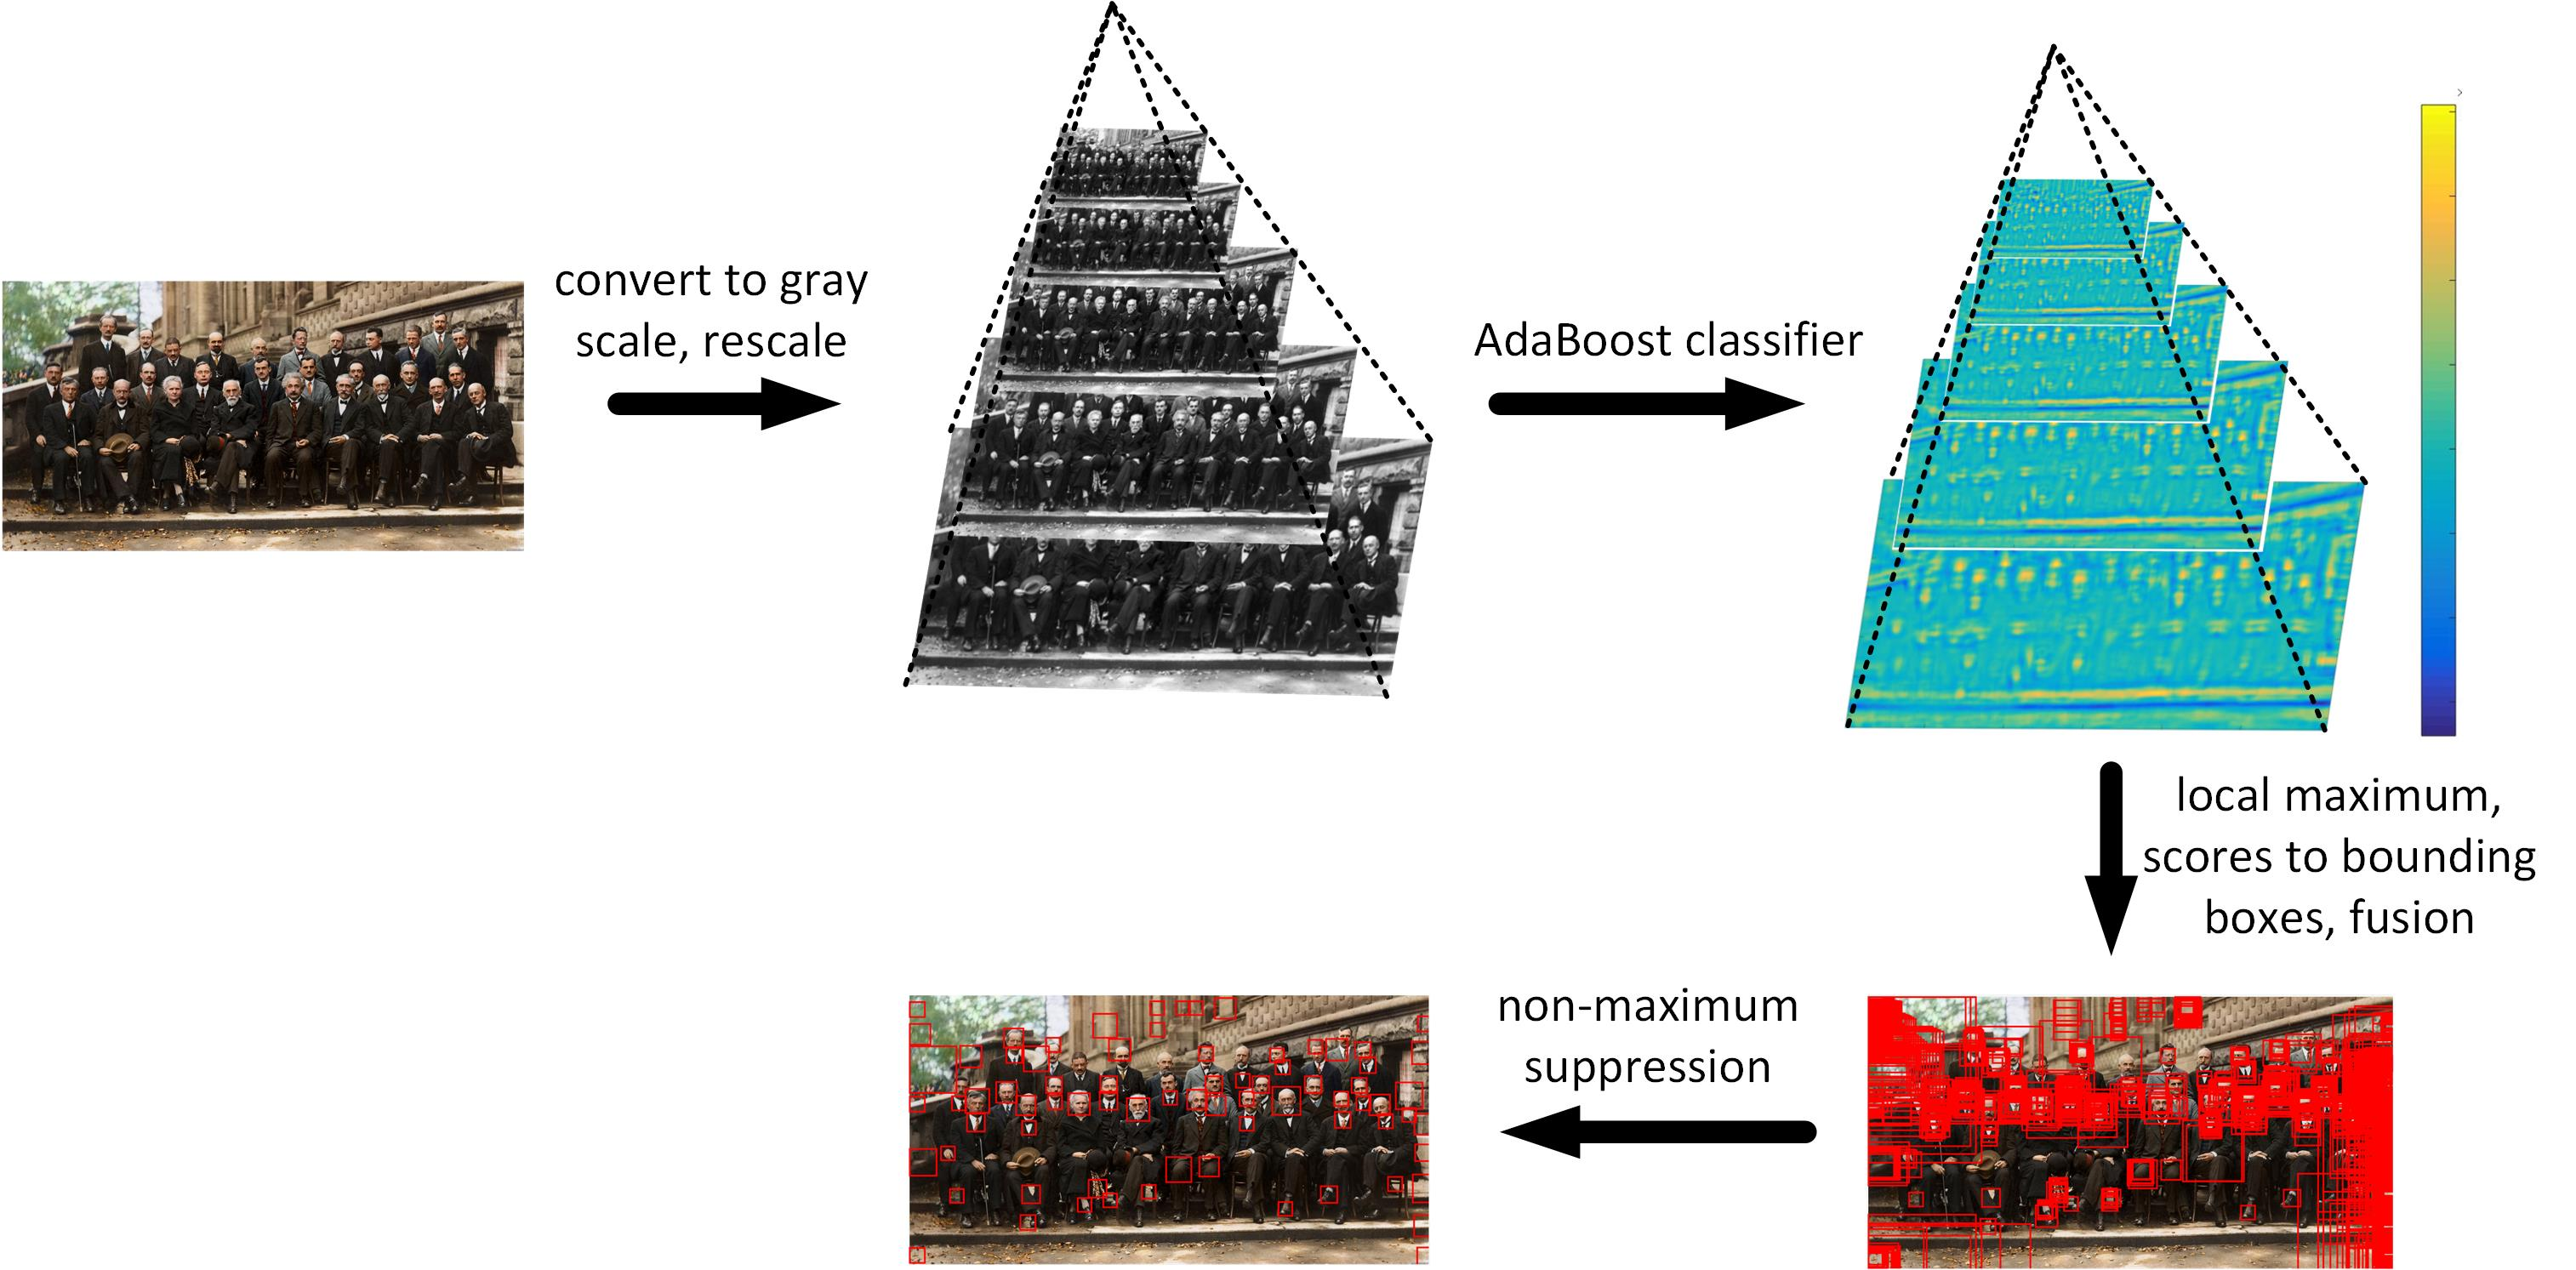
\includegraphics[scale=0.3]{figs/pipeline.jpg}
%     \caption{Pipeline for Face Detection.}
%     \label{pipeline}
% \end{figure}

% It would be more intuitive in fig. \ref{pipeline}. In this homework, step 3 and 5 is provided through two matlab functions that you can find in \texttt{h2materials/problem2/utils}:
% \begin{itemize}
%     \item \texttt{get\_localmax}: This function return the locations which may have a face. The candidate locations must be the local maximum, and their scores are greater than a pre-defined threshold.
%     \item \texttt{nms}: This function implements non maximum suppression (NMS), a post-processing algorithm for merging the bounding boxes that belong to the same face. For each loop, it takes a bounding box with highest score, and removes the rest of bounding boxes that overlap with it.
% \end{itemize}

% Details about inputs and outputs can be found on the corresponding files.


% You need to \ul{implement step 1, step 2, and step 4, and build the entire face detection system.} 

% To test your system, 4 images are provided in the directory \texttt{hw2materials/problem2/photos}. \ul{Using these images, show your best results and the running times in the report.} You are allowed to tune different parameters (number of eigenfaces, number of weak learners, threshold, etc). The result should be in the form of image with the predicted bounding boxes.

